\chapter{Reconnaissance faciale}
\label{ch:reco_faciale}

Une partie critique du projet consiste à pouvoir identifier des personnes en fonction des images capturées par la
caméra. La reconnaissance faciale étant un sujet d’étude très complexe, il sera nécessaire d’utiliser des solutions
clés en main afin de pouvoir l’incorporer dans l’ensemble du projet. Il peut toutefois être intéressant de
comprendre les bases et les implications de cette technologie.

\subsection{Une petite touche de théorie}
La reconnaissance faciale utilise la technologie du Machine Learning, et plus précisement du Deep Learning.
Le principe consite à l’extraction de données intéressantes d’une image (les caractérstiques) afin de créer ou lier une
« empreinte biométrique » à un visage. Ce processus est exemplifié dans la figure ~\ref{fig:reco-process} . Par exemple en mesurant l’écartement des yeux, la longeur du nez, la
profondeur des orbites, on obtient des données uniques qui permettront d’identifier la même personne sur une
image différente.

Les cas d’utilisation de la reconnaissance faciale sont nombreux.
En voici une liste non-exhaustive :
\begin{itemize}
\item Identifier l’utilisateur d’un téléphone (Apple FaceID)
\item Aide à la recherche des personnes disparues
\item Aide aux personnes malvoyantes (détection et notification du sourire de ces interlocteurs)
\item Labellisation des personnes sur les réseaux sociaux
\item Lutte contre le terrorisme
\end{itemize}

\begin{figure}[H]
	\centering
	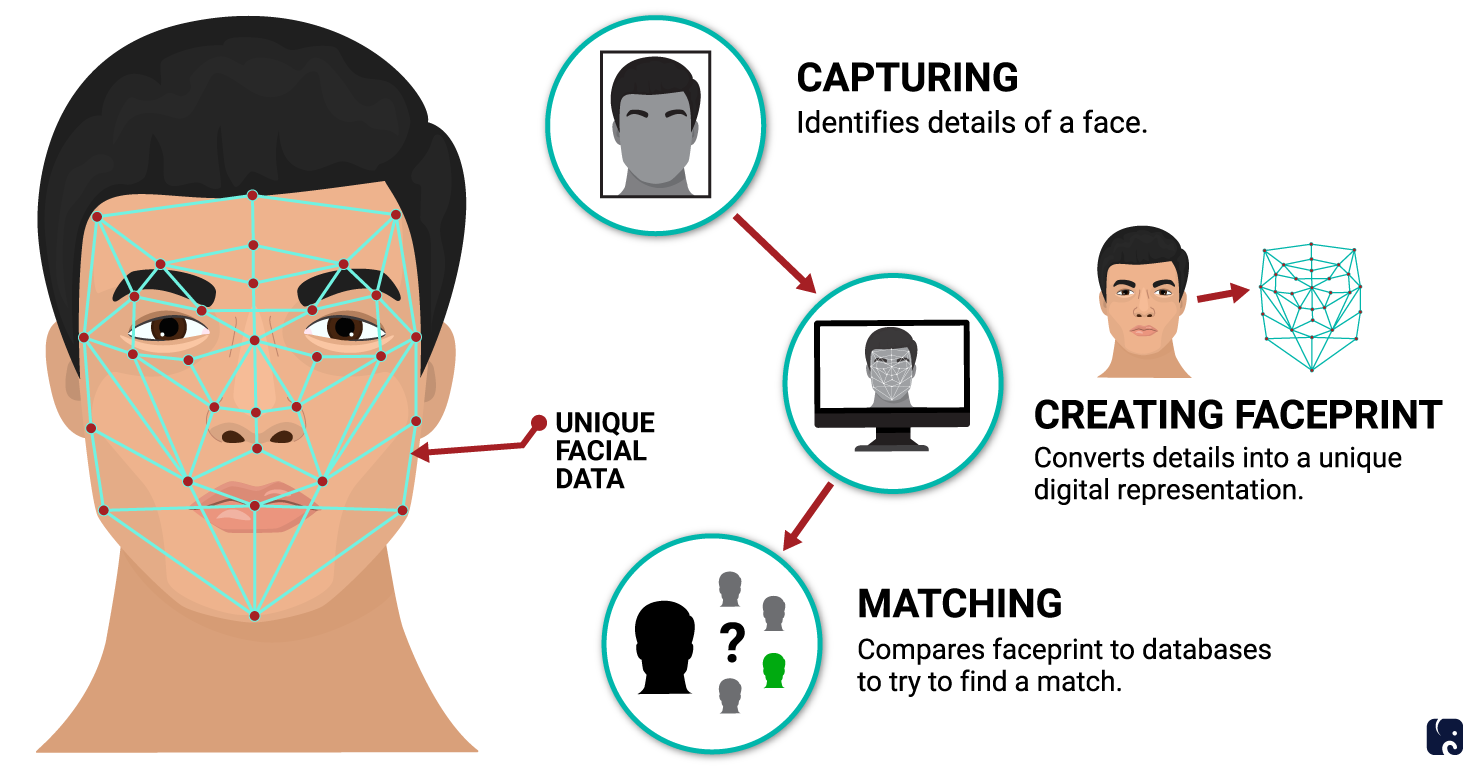
\includegraphics[width=12cm]{images/proto-5.png}
	\caption{Processus de reconnaissance faciale}
	\label{fig:reco-process}
\end{figure}

\section{Choix de la solution}

À l'aide de quelques valeurs clés (précision, rappel, nombre de faux-positifs, ...) nous allons comparer plusieurs solutions existantes et "clés en main" de reconnaissance faciale.
La figure ~\ref{fig:tab-comparatif-reco} ci-dessous énumère les fonctionnalités offertes par les diverses solutions du marché.

\begin{figure}[H]
	\centering
	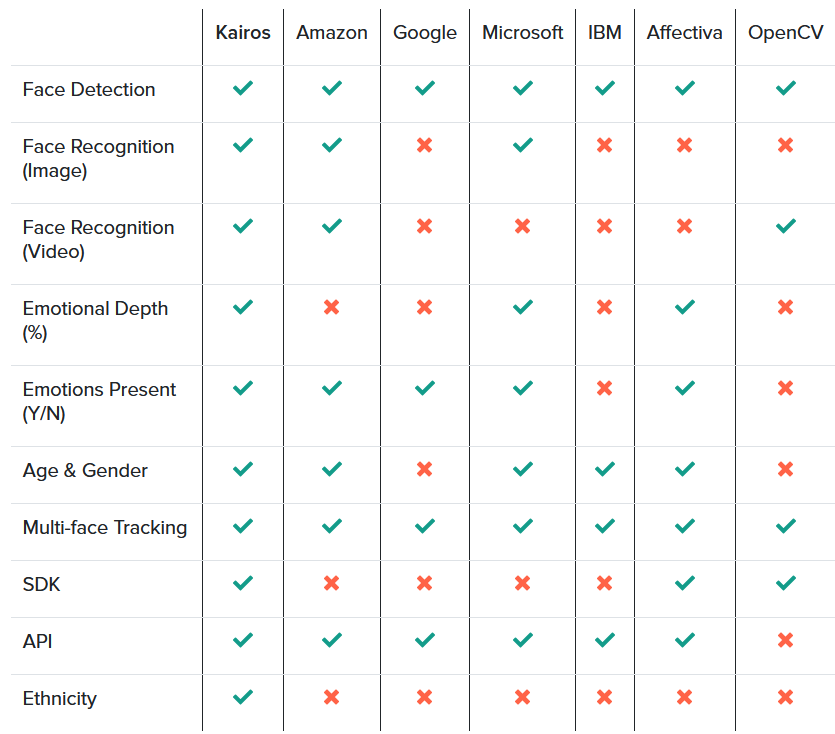
\includegraphics[width=12cm]{images/proto-4.png}
	\caption{Tableau comparatif de solution de reconnaissance faciale}
	\label{fig:tab-comparatif-reco}
\end{figure}

Ce qui est nécessaire, c’est la « Face recognition » sur image (plus compatible avec la notion d’IoT qu’un flux vidéo
complet.) Les trois solutions le proposant sont :

\begin{itemize}
\item Kairos
\item Amazon AWS : Rejognition
\item Microsoft Azure : Face
\end{itemize}

Trois facteurs sont alors importants dans le cadre du projet : La précision, le prix et la facilité d’utilisation.

\subsection{Performances}
Concernant la précision, on peut le mesure à l’aide des concepts de True Positive (Un visage est correctement
identifié), True Negative (Un visage est correctement exclu), False Positive (Un visage est identifié en tant qu’un
autre) et False Negative (Un visage n’a pas été identifié comme connu)

Une source a utilisé un dataset de visage de l’université de Essex afin de mesurer ces valeurs dans différents
contextes pour les trois solutions. Voici les résultats principaux.

\begin{itemize}
\item Precision (TP/(TP+FP)
\item Recall (TP/(TP+FN))
\end{itemize}

\begin{table}[H]
\small
\begin{tabular}{|m{2cm} | m{2cm} | m{2cm} | m{2cm} |m{2cm} |m{2cm} |m{2cm}|}
\hline
{\color[HTML]{000000} \textbf{Provider}}              & {\color[HTML]{000000} \textbf{TP}} & {\color[HTML]{000000} \textbf{FP}} & {\color[HTML]{000000} \textbf{TN}} & {\color[HTML]{000000} \textbf{FN}} & {\color[HTML]{000000} \textbf{Precision}} & {\color[HTML]{000000} \textbf{Recall}} \\ \hline
{\color[HTML]{000000} AWS rekognition}                & {\color[HTML]{000000} 149}                    & {\color[HTML]{000000} 0}                       & {\color[HTML]{000000} 150}                    & {\color[HTML]{000000} 1}                       & {\color[HTML]{000000} 100\%}                            & {\color[HTML]{000000} 99.3\%}                        \\ \hline
{\color[HTML]{000000} Microsoft cognitive   services} & {\color[HTML]{000000} 131}                    & {\color[HTML]{000000} 0}                       & {\color[HTML]{000000} 150}                    & {\color[HTML]{000000} 19}                      & {\color[HTML]{000000} 100\%}                            & {\color[HTML]{000000} 87.3\%}                        \\ \hline
{\color[HTML]{000000} Kairos}                         & {\color[HTML]{000000} 108}                    & {\color[HTML]{000000} 0}                       & {\color[HTML]{000000} 150}                    & {\color[HTML]{000000} 42}                      & {\color[HTML]{000000} 100\%}                            & {\color[HTML]{000000} 72\%}                          \\ \hline
\end{tabular}
\caption{Seuil de confiance AWS rekognition: 95\% Microsoft: 80\% Kairos: 95\%}
\end{table}

\begin{table}[H]
\begin{tabular}{|m{2cm} | m{2cm} | m{2cm} | m{2cm} |m{2cm} |m{2cm} |m{2cm}|}
\hline
{\color[HTML]{000000} \textbf{Provider}}              & {\color[HTML]{000000} \textbf{TP}} & {\color[HTML]{000000} \textbf{FP}} & {\color[HTML]{000000} \textbf{TN}} & {\color[HTML]{000000} \textbf{FN}} & {\color[HTML]{000000} \textbf{Precision}} & {\color[HTML]{000000} \textbf{Recall}} \\ \hline
{\color[HTML]{000000} AWS rekognition}                & {\color[HTML]{000000} 150}                    & {\color[HTML]{000000} 2}                       & {\color[HTML]{000000} 148}                    & {\color[HTML]{000000} 0}                       & {\color[HTML]{000000} 98.7\%}                          & {\color[HTML]{000000} 100\%}                        \\ \hline
{\color[HTML]{000000} Microsoft cognitive   services} & {\color[HTML]{000000} 137}                    & {\color[HTML]{000000} 0}                       & {\color[HTML]{000000} 150}                    & {\color[HTML]{000000} 13}                      & {\color[HTML]{000000} 100\%}                           & {\color[HTML]{000000} 91.3\%}                       \\ \hline
{\color[HTML]{000000} Kairos}                         & {\color[HTML]{000000} 148}                    & {\color[HTML]{000000} 0}                       & {\color[HTML]{000000} 150}                    & {\color[HTML]{000000} 2}                       & {\color[HTML]{000000} 100\%}                           & {\color[HTML]{000000} 98.7\%}                       \\ \hline
\end{tabular}
\caption{Seuil de confiance AWS rekognition 70\% Microsoft: 50\% Kairos: 70\%}
\end{table}

\begin{table}[H]
\begin{tabular}{|m{2cm} | m{2cm} | m{2cm} | m{2cm} |m{2cm} |m{2cm} |m{2cm}|}
\hline
{\color[HTML]{000000} \textbf{Provider}}              & {\color[HTML]{000000} \textbf{TP}} & {\color[HTML]{000000} \textbf{FP}} & {\color[HTML]{000000} \textbf{TN}} & {\color[HTML]{000000} \textbf{FN}} & {\color[HTML]{000000} \textbf{Precision}} & {\color[HTML]{000000} \textbf{Recall}} \\ \hline
{\color[HTML]{000000} AWS rekognition}                & {\color[HTML]{000000} 150}                    & {\color[HTML]{000000} 2}                       & {\color[HTML]{000000} 148}                    & {\color[HTML]{000000} 0}                       & {\color[HTML]{000000} 98.7\%}                          & {\color[HTML]{000000} 100\%}                        \\ \hline
{\color[HTML]{000000} Microsoft cognitive   services} & {\color[HTML]{000000} 137}                    & {\color[HTML]{000000} 10}                      & {\color[HTML]{000000} 140}                    & {\color[HTML]{000000} 13}                      & {\color[HTML]{000000} 93.2\%}                          & {\color[HTML]{000000} 91.3\%}                       \\ \hline
{\color[HTML]{000000} Kairos}                         & {\color[HTML]{000000} 150}                    & {\color[HTML]{000000} 19}                      & {\color[HTML]{000000} 131}                    & {\color[HTML]{000000} 0}                       & {\color[HTML]{000000} 88.7\%}                          & {\color[HTML]{000000} 100\%}                        \\ \hline
\end{tabular}
\caption{Seuil de confiance AWS rekognition: 50\% Microsoft: 30\% Kairos: 50\%}
\end{table}

Parmi ces résultats, nous pouvons voir que rekognition se démarque par son absence presque totale de FN et un
taux faible de faux positifs, même avec un seuil de confiance bas (ce qui est un avantage dans un environnement
moyennement précis tel que la raspberry).

\subsection{Tarification}

Concernant la tarfication, Amazon et Microsoft se démarquent de Kairos grâce à leur prix moins élevés, et à des
solutions gratuites.

\subsubsection{Kairos}

Kairos pratique des prix mensuels fixes ainsi qu’un supplément par transaction. Par exemple, l’offre « Student
Cloud » coûte 19\$ par mois + 0.02\$ par transaction, avec tout de fois 2 semaines d’essai gratuites.

\subsubsection{Microsoft Azure Face}

Microsoft propose deux solutions : « Free - Web/Container » et « Standard - Web/Container ». Il est à noter que la
tier gratuit ne comprend pas le « Face Storage » et que l’entraînement est compté dans les transactions (1
transaction / 1000 images utilisées pendant l’entrainement)

\begin{table}[]
\small
\begin{tabular}{|
>{\columncolor[HTML]{FFFFFF}}m{2cm} |
>{\columncolor[HTML]{FFFFFF}}m{2cm} |
>{\columncolor[HTML]{FFFFFF}}m{3cm} |
>{\columncolor[HTML]{FFFFFF}}m{8cm} |}
\hline
{\color[HTML]{000000} \textbf{Instance}}                                                  & {\color[HTML]{000000} \textbf{Transactions Per Second    (TPS) *}}      & {\color[HTML]{000000} \textbf{Features}}                                                                                                                                  & {\color[HTML]{000000} \textbf{Price}}                                                                                                                                                                                                                                                 \\ \hline
{\color[HTML]{000000} Free}                                               & {\color[HTML]{000000} 20 transactions per   minute}                     & {\color[HTML]{000000} \begin{tabular}[c]{@{}l@{}}Face Detection\\    Face Verification\\    Face Identification\\    Face Grouping\\    Similar Face Search\end{tabular}} & {\color[HTML]{000000} 30,000 transactions free   per month}                                                                                                                                                                                                                           \\ \hline
\cellcolor[HTML]{FFFFFF}{\color[HTML]{000000} }                                           & \cellcolor[HTML]{FFFFFF}{\color[HTML]{000000} }                         & {\color[HTML]{000000} \begin{tabular}[c]{@{}l@{}}Face Detection\\    Face Verification\\    Face Identification\\    Face Grouping\\    Similar Face Search\end{tabular}} & {\color[HTML]{000000} \begin{tabular}[c]{@{}l@{}}0-1M transactions - \$1   per 1,000 transactions\\    1M-5M transactions - \$0.80 per 1,000 transactions\\    5M-100M transactions - \$0.60 per 1,000 transactions\\    100M+ transactions - \$0.40 per 1,000 transactions\end{tabular}} \\ \cline{3-4} 
\multirow{-2}{*}{\cellcolor[HTML]{FFFFFF}{\color[HTML]{000000} Standard}} & \multirow{-2}{*}{\cellcolor[HTML]{FFFFFF}{\color[HTML]{000000} 10 TPS}} & {\color[HTML]{000000} Face Storage}                                                                                                                                       & {\color[HTML]{000000} \$0.01 per 1,000 faces per   month}                                                                                                                                                                                                                             \\ \hline
\end{tabular}
\end{table}

\subsubsection{Amazon AWS rekognition}
Rekognizion est compris dans l’offre gratuite d’AWS durant les 12 premiers mois d’utilisation et ce pour 5'000
transaction ainsi que 1'000 métadonnées par mois.

\begin{table}[]
\small
\begin{tabular}{|m{6cm}|m{3cm}|m{4cm}|l}
\cline{1-3}
{\color[HTML]{000000} \textbf{Type de coût}}                           & {\color[HTML]{000000} \textbf{Tarification}} & {\color[HTML]{000000} \textbf{Prix pour    1 000 images}} &  \\ \cline{1-3}
{\color[HTML]{000000} Premier million d'images traitées par mois}      & {\color[HTML]{000000} 0,001 USD par image}   & {\color[HTML]{000000} 1,00 USD}                           &  \\ \cline{1-3}
{\color[HTML]{000000} 9 millions d'images traitées suivants par mois}  & {\color[HTML]{000000} 0,0008 USD par image}  & {\color[HTML]{000000} 0,80 USD}                           &  \\ \cline{1-3}
{\color[HTML]{000000} 90 millions d'images traitées suivants par mois} & {\color[HTML]{000000} 0,0006 USD par image}  & {\color[HTML]{000000} 0,60 USD}                           &  \\ \cline{1-3}
{\color[HTML]{000000} Plus de 100 millions d'images traitées par mois} & {\color[HTML]{000000} 0,0004 USD par image}  & {\color[HTML]{000000} 0,40 USD}                           &  \\ \cline{1-3}
\end{tabular}
\end{table}

\subsection{Facilité d’utilisation}
Concernant la facilité d’utilisation, une documentation de bonne qualité semble disponible pour Microsoft et
Amazon. Toutefois, il semble très important pour Microsoft d’avoir des photos d’entraînements avant le processus
de reconnaissance, ce qui ne répond pas au cahier des charges.

\subsection{Choix de la solution}
Grâce aux différents facteurs analysés, c’est la solution d’Amazon (Rekognition) qui a été retenue pour ce projet. À
l’aide d’un tiers gratuit (majoritairement suffisant pour la période de développement), de très bonnes performances
et d’un use case compatible avec le cahier des charges, nous pouvons affirmer qu’il est pertinent de faire ce choix.

\section{Amazon Rekognition : présentation}
Comme expliqué précédemment, Amazon rekognition est un service de reconnaissance d’images. Bien que nous
utilisons seulement les fonctionnalités concernant les visages, il est aussi possible par exemple d’identifier du texte,
des objets ou encore des images inappropriées (contenu explicite et suggestif).

\subsection{Concepts et opérations}
Pour pouvoir utiliser Rekognition, il faut connaître les opérations principales de l’API et en comprendre les concepts
principaux.

\underline{Features} (caractéristique) : En machine learning, les caractéristiques sont les variables d’entrées permettant de
simplifier le problème et sur lesquelles nous allons nous baser pour faire des classifications. Par exemple, pour la
détection de visages, certaines des caractéristiques sont : écartement des yeux, couleur des yeux, la longueur du
nez, la forme des joues, la profondeur des orbites, ou encore la largeur de la mâchoire. La combinaison de ces
caractéristiques permettent souvent d’identifier de manière unique un individu.

\underline{Collection} : Les collections sont des « conteneurs » AWS server-side qui rassemblent les informations (métadata)
des visages ajoutés. Une collection est identifiée par un ARN (Amazon Resource Name) unique et peut être créée
grâce à l’opération « CreateCollection »

\underline{IndexFace} : Opération d’ajout d’un ou plusieurs visages (métadatas) dans une collection. En entrée, il faut
principalement une image (blob), le nom de la collection dans laquelle insérer les visages, le nombre maximum de
visages à indexer (les visages sont indexés du plus petit au plus grand. Ainsi, sur une image contenant 5 personnes,
si le paramètre vaut 2, seulement les 2 plus grand visages seront ajoutés à la collection)

\underline{SearchFacesByImage}\label{text:SearchFacesByImage} : Opération prenant une image en entrée, récupère le visage le plus visible et cherche dans
une collection donnée si ce visage est reconnu. Si c’est le cas, on peut alors inférer que l’image représente la même
personne que les métadonnées correspondantes.

La figure~\ref{fig:reko-workflow} présente un workflow détaillé d’Amazon Rekognition

\begin{figure}[H]
	\centering
	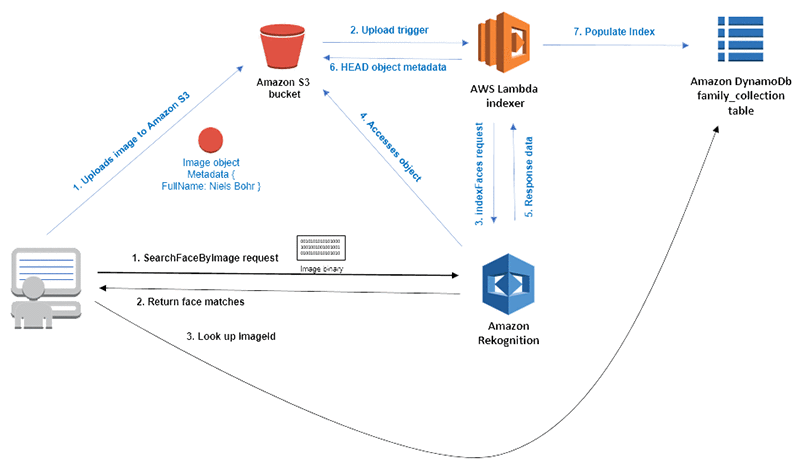
\includegraphics[width=12cm]{images/proto-6.png}
	\caption{Workflow d'Amazon Rekognition}
	\label{fig:reko-workflow}
\end{figure}

\subsection{Prérequis}

Afin de pouvoir travailler avec Amazon Rekognizion, il est nécessaire d’avoir une clé d’authentification à leur API.
Pour cela, il faut créer un compte et s’inscrire au service. Une fois la clé obtenue, nous allons utiliser leur SDK pour
Python : boto3  et leur CLI : awscli grâce auquel nous pouvons effectuer la configuration de base.
Avec la comande `aws configure` nous pouvons saisir la clé qui sera alors utilisée pendant nos appels d’API.

\begin{listingsbox}{console}{Configuration du client amazon}
aws configure
AWS Access Key ID [None]:  YOUR_ACCESS_KEY_ID
AWS Secret Access Key [None]: YOUR_SECRET_ACCESS_KEY
Default region name [None]: us-east-1
Default output format [None]: ENTER
\end{listingsbox}